%%%%%%%%%%%%%%%%%%%%%%%%%%%%%%%%%%%%%%%%%%%%%%%%%%%%%%%%%%%%%%%%%%%%%
%%                                                                 %%
%% Please do not use \input{...} to include other tex files.       %%
%% Submit your LaTeX manuscript as one .tex document.              %%
%%                                                                 %%
%% All additional figures and files should be attached             %%
%% separately and not embedded in the \TeX\ document itself.       %%
%%                                                                 %%
%%%%%%%%%%%%%%%%%%%%%%%%%%%%%%%%%%%%%%%%%%%%%%%%%%%%%%%%%%%%%%%%%%%%%

%%\documentclass[referee,sn-basic]{sn-jnl}% referee option is meant for double line spacing

%%=======================================================%%
%% to print line numbers in the margin use lineno option %%
%%=======================================================%%

%%\documentclass[lineno,sn-basic]{sn-jnl}% Basic Springer Nature Reference Style/Chemistry Reference Style

%%======================================================%%
%% to compile with pdflatex/xelatex use pdflatex option %%
%%======================================================%%

%%\documentclass[pdflatex,sn-basic]{sn-jnl}% Basic Springer Nature Reference Style/Chemistry Reference Style

%%\documentclass[sn-basic]{sn-jnl}% Basic Springer Nature Reference Style/Chemistry Reference Style
%%\documentclass[sn-mathphys]{sn-jnl}% Math and Physical Sciences Reference Style
%%\documentclass[sn-aps]{sn-jnl}% American Physical Society (APS) Reference Style
\documentclass[sn-vancouver]{sn-jnl}% Vancouver Reference Style
%%\documentclass[sn-apa]{sn-jnl}% APA Reference Style
%%\documentclass[sn-chicago]{sn-jnl}% Chicago-based Humanities Reference Style
%%\documentclass[sn-standardnature]{sn-jnl}% Standard Nature Portfolio Reference Style
%%\documentclass[default]{sn-jnl}% Default
%%\documentclass[default,iicol]{sn-jnl}% Default with double column layout

%%%% Standard Packages
%%<additional latex packages if required can be included here>
\usepackage[scaled]{beramono}
\usepackage[T1]{fontenc}
%%%%

%%%%%=============================================================================%%%%
%%%%  Remarks: This template is provided to aid authors with the preparation
%%%%  of original research articles intended for submission to journals published 
%%%%  by Springer Nature. The guidance has been prepared in partnership with 
%%%%  production teams to conform to Springer Nature technical requirements.
%%%%  Editorial and presentation requirements differ among journal portfolios and 
%%%%  research disciplines. You may find sections in this template are irrelevant 
%%%%  to your work and are empowered to omit any such section if allowed by the 
%%%%  journal you intend to submit to. The submission guidelines and policies 
%%%%  of the journal take precedence. A detailed User Manual is available in the 
%%%%  template package for technical guidance.
%%%%%=============================================================================%%%%

\jyear{2022}%

%% as per the requirement new theorem styles can be included as shown below
\theoremstyle{thmstyleone}%
\newtheorem{theorem}{Theorem}% meant for continuous numbers
%%\newtheorem{theorem}{Theorem}[section]% meant for sectionwise numbers
%% optional argument [theorem] produces theorem numbering sequence instead of independent numbers for Proposition
\newtheorem{proposition}[theorem]{Proposition}% 
%%\newtheorem{proposition}{Proposition}% to get separate numbers for theorem and proposition etc.

\theoremstyle{thmstyletwo}%
\newtheorem{example}{Example}%
\newtheorem{remark}{Remark}%

\theoremstyle{thmstylethree}%
\newtheorem{definition}{Definition}%

\raggedbottom
%%\unnumbered% uncomment this for unnumbered level heads

\begin{document}

%SJ: ik wil graag dat semantiek centraal staat in de titel. Ook de woorden "Modeling convention" en "ArchiMate" horen in de titel.
\title{Enhancing ArchiMate wih Semantic Modeling Conventions}
% use \title[short title]{long title} to get a shorter title above all but the first pages.

%%=============================================================%%
%% Prefix	-> \pfx{Dr}
%% GivenName	-> \fnm{Joergen W.}
%% Particle	-> \spfx{van der} -> surname prefix
%% FamilyName	-> \sur{Ploeg}
%% Suffix	-> \sfx{IV}
%% NatureName	-> \tanm{Poet Laureate} -> Title after name
%% Degrees	-> \dgr{MSc, PhD}
%% \author*[1,2]{\pfx{Dr} \fnm{Joergen W.} \spfx{van der} \sur{Ploeg} \sfx{IV} \tanm{Poet Laureate} 
%%                 \dgr{MSc, PhD}}\email{iauthor@gmail.com}
%%=============================================================%%

\author[1]{\fnm{Stef} \sur{Joosten}}\email{Stef.Joosten@ou.nl}

\author[2]{\fnm{Ella} \sur{Roubtsova}}\email{Ella.Roubtsova@ou.nl}
%\equalcont{These authors contributed equally to this work.}



\affil[1,2]{\orgdiv{Faculty of Science}, \orgname{Open University}, \orgaddress{\street{Valkenburgerweg 177}, \city{Heerlen}, \postcode{6419 AT}, \country{Netherlands}}}
\affil[1]{\orgdiv{Architecture Dept.}, \orgname{Ordina}, \orgaddress{\street{Ringwade 1}, \city{Nieuwegein}, \postcode{3439 LM}, \country{Netherlands}}}


%%==================================%%
%% sample for unstructured abstract %%
%%==================================%%
\abstract{This paper investigates the use of modeling conventions for enterprise models.
It proposes to use Ampersand to enhance ArchiMate with semantics,
making ArchiMate models more useful in practice.
For enterprise architects who want more from ArchiMate than just drawing pictures,
this paper proposes to use a language and a tool, Ampersand, to impose and verify modeling conventions in ArchiMate models.
Unlike informal languages, Ampersand allows enterprise architects to signal where an ArchiMate model violates their own modeling conventions,
so they can fix the model accordingly.
It allows enterprise architects to enhance their ArchiMate models with semantic claims that are proven by Ampersand.
This paper contains a case study that demonstrates the approach.
The authors also share their experience in making the case study, showing a way to achieve relevant results.
}

%%================================%%
%% Sample for structured abstract %%
%%================================%%

% \abstract{\textbf{Purpose:} The abstract serves both as a general introduction to the topic and as a brief, non-technical summary of the main results and their implications.
% The abstract must not include subheadings (unless expressly permitted in the journal's Instructions to Authors), equations or citations. As a guide the abstract should not exceed 200 words. Most journals do not set a hard limit however authors are advised to check the author instructions for the journal they are submitting to.
% 
% \textbf{Methods:} The abstract serves both as a general introduction to the topic and as a brief, non-technical summary of the main results and their implications. The abstract must not include subheadings (unless expressly permitted in the journal's Instructions to Authors), equations or citations. As a guide the abstract should not exceed 200 words. Most journals do not set a hard limit however authors are advised to check the author instructions for the journal they are submitting to.
% 
% \textbf{Results:} The abstract serves both as a general introduction to the topic and as a brief, non-technical summary of the main results and their implications. The abstract must not include subheadings (unless expressly permitted in the journal's Instructions to Authors), equations or citations. As a guide the abstract should not exceed 200 words. Most journals do not set a hard limit however authors are advised to check the author instructions for the journal they are submitting to.
% 
% \textbf{Conclusion:} The abstract serves both as a general introduction to the topic and as a brief, non-technical summary of the main results and their implications. The abstract must not include subheadings (unless expressly permitted in the journal's Instructions to Authors), equations or citations. As a guide the abstract should not exceed 200 words. Most journals do not set a hard limit however authors are advised to check the author instructions for the journal they are submitting to.}

%Keywords sorted alphabetically
\keywords{Ampersand,  ArchiMate, Automated Constraint Verification, Enterprise Architecture, Formal Methods, Modeling Convention, Relation Algebra}

%%\pacs[JEL Classification]{D8, H51}

%%\pacs[MSC Classification]{35A01, 65L10, 65L12, 65L20, 65L70}

\maketitle

\section{Introduction}\label{sec1}
This article is an extended version of the conference paper presented at the International Conference on Enterprise Information Systems ICEIS-2022~\cite{iceis22}.
The Open Group language ArchiMate~\cite{ArchiMate} is a popular language for enterprise modeling.
Many tools support ArchiMate, e.g. Sparx, BizzDesign, Archi.
These tools limit model checking to stating whether a relationship between two graphical elements is allowed or not, based on their types.
As a consequence, ArchiMate is typically used for diagramming purposes only.

The ArchiChecker project was conducted at the Open University of the Netherlands to enhance ArchiMate with semantic constraints in a proper formal notation.
We want to facilitate enterprise architects to define their modeling conventions in a direct, mathematically sound way.
The authors believe this will yield better enterprise models, which we demonstrate by a case study in this paper.

In this research we focus on semantic constraints that represent modeling conventions,
so that a computer can determine where these constraints are violated in an ArchiMate model.
We focus on semantic rather than syntactic constraints because we aim for added value in the domain in which architects work.
We focus on modeling conventions that constrain the modeling space, so we can use tooling alongside of the modeling tool.
We focus on computing violations because that makes the work concrete enough to have an impact in practice.

Several authors have noticed that the modeling conventions and semantic constraints
form a real challenge in enterprise architecture~\cite{kharlamov2016capturing,chatzikonstantinou2012policy,ramos2014automated,bider2020structural}.
However, tool support is often limited, forcing enterprise architects to write plugins (e.g.~jArchi),
This forces enterprise architects to write program code (e.g.~JavaScript in case of jArchi).
Babkin and Ponomarev~\cite{babkin2017analysis} form a noteworthy exception.
They have taken a similar approach as ours, but they do not report any practical experience with it.
They too have picked a language based on relation algebra, Alloy~\cite{Alloy2006}, in which they write semantic constraints.

In an earlier exploratory study~\cite{iceis22}, we questioned architects from the University Medical Center in Utrecht about their modeling conventions,
hoping to formalize them as constraints and provide added value by verifying them.
Although it all worked, the architects did not come up with very relevant modeling conventions.
After a fair amount of workshops and discussions, about ten modeling conventions remained.
Since we failed to focus sufficiently on relevance, this study only showed that the principle of checking modeling conventions works in a practical situation.
Consequently, the violations that resulted from checking the modeling conventions were not very relevant either.

In the current study, we have tried a different approach.
We proposed rather than elicited the modeling conventions,
resulting in more relevant results.
Enterprise architects understand the violations and may or may not find them relevant.
They are more likely to change or enhance their models to resolve the violations.
It leads to enterprise models with verified semantic claims.

This paper is built up as follows
\begin{itemize}
\item Chapter~\ref{Prerequisites} discusses three claims that are prerequiste for this study:
\item
Section~\ref{ArchiMate} gives an overview of the language ArchiMate, showing that the metamodel of ArchiMate enables automated constraint verification.
\item
Section~\ref{Constraints} presents the results of a literature study, which shows that the need to enhance ArchiMate with semantic constraints is acknowledged by the scientific community.
\item
Section~\ref{Verif} discusses the existing attempts of automated verification of constraints in ArchiMate models.
\item
Section~\ref{toolset} discusses the method of verifying constraints by presenting the Ampersand compiler in the context of analyzing an ArchiMate model.
This section proposes a practical approach to formalise modeling conventions by constraints and let Ampersand compute violations of these constraints.
\item
Section~\ref{host families} reports a summary of a case study to illustrate the approach in a realistic situation.
\item
Section~\ref{reflection} reflects on the case study and the lessons learned from it.
\item
Section~\ref{conclusion} concludes the paper and draws on future work.
\end{itemize}

%\section{Results}\label{sec2}
\section{Prerequisites}\label{Prerequisites}
The contribution of our paper is to illustrate the relevance of automated constraint verification in ArchiMate models by means of a case study.
Before that, we must establish three claims, each of which is elaborated in a separate section.
\begin{itemize}
   \item The metamodel of ArchiMate makes ArchiMate models suitable for automated analysis (sct.~\ref{ArchiMate}).
   \item Scientific work on the modeling of constraints in ArchiMate has yielded no results suitable for automated verification (sct.~\ref{Constraints}).
   \item Automated constraint verification is applicable to ArchiMate, but not practiced a lot (sct.~\ref{Verif}).
\end{itemize}

\subsection{ArchiMate}\label{ArchiMate}
To understand how constraints can be imposed on ArchiMate models,
let us briefly summarize the ArchiMate language.
Figure~\ref{how} shows a screenshot of the open source tool Archi~\cite{beauvoir2018archi}, which we have used throughout this study.

\begin{figure}[hbtp]
 \centering
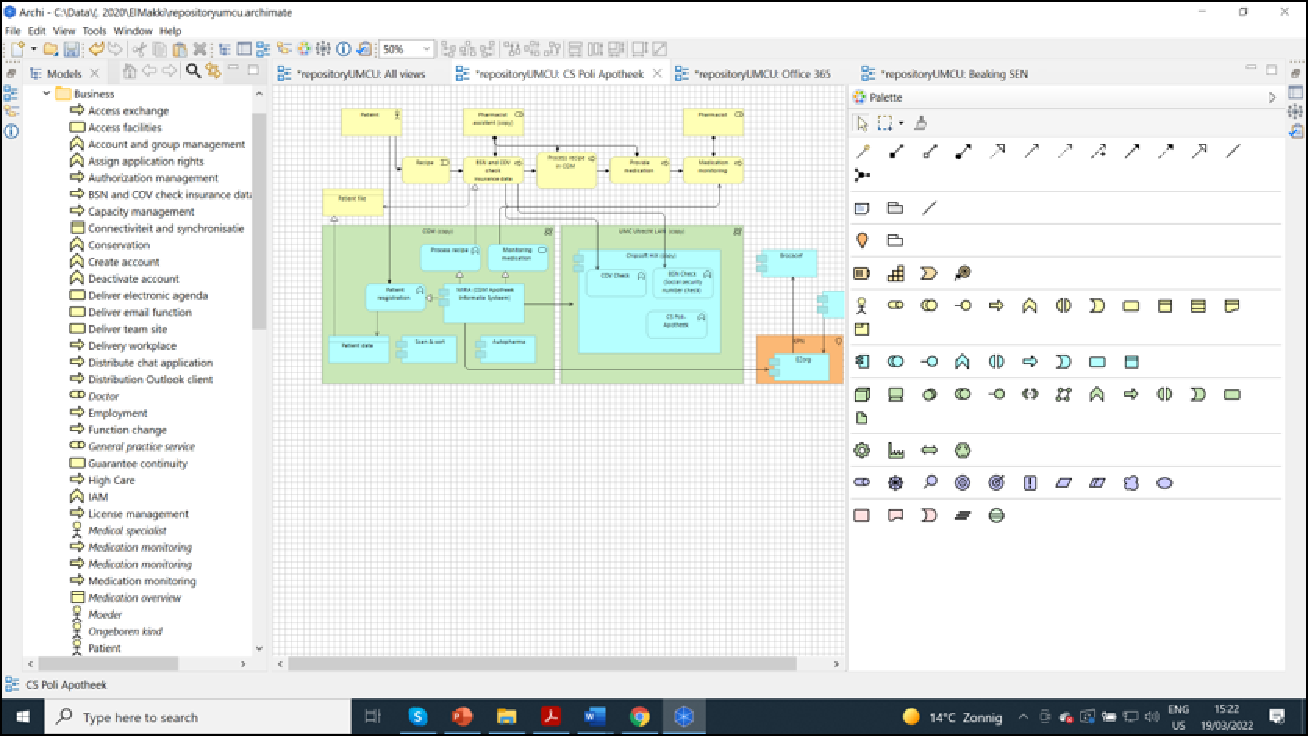
\includegraphics[clip=true, scale=0.5]{HowArchitectWorks}
\caption{How an architect works in ArchiMate}
\label{how}   % Give a unique label
\end{figure}

The ArchiMate metamodel~\cite{ArchiMateMetaModel} offers a set of elements and relationships.
Elements are ``used to define and describe the constituent parts of Enterprise Architectures and their unique set of characteristics''~\cite{ArchiMate}.
Relationships represent connections between source and target elements.
Each element and each relationship has its own shape, to be picked by the modeler from a limited set of shapes,
in the palette on the right hand side of figure~\ref{how}.
Each shape reflects the type of the element or relationship.
The meaning of each shape is described in natural language in the ArchiMate reference document~\cite{ArchiMate}.

Throughout this document we use the word ``model'' in the meaning used by ArchiMate~\cite{ArchiMate},
which contains a collection of views. Each view is one diagram.
So an ArchiMate model contains a collection of diagrams (views) as opposed to the more conventional meaning in which a model refers to one diagram only.
In each single view, ArchiMate shows a set of boxes presenting instances of elements and lines between those boxes, presenting instances of relationships.
So the user perceives every view as a graphical diagram (the central part in figure~\ref{how}) that shows details of the entire ArchiMate model.

The internal data structure in ArchiMate (shown in the panel on the left hand side of figure~\ref{how}) contains
\begin{itemize}
  \item a collection of instances of elements,
  \item a collection of instances of relationships, and
  \item a collection of views in which the instances of elements and relationships are shown.
\end{itemize}
An attractive characteristic of ArchiMate is that different views can share the same instances of elements and relationships.
One element instance can even have different shapes in different views,
but still be the same\footnote{The notion of ``the same'' is not defined in the ArchiMate reference document~\cite{ArchiMate},
but ArchiMate tools typically use an internal key to identify elements.} instance.
A useful consequence is that changing a name of an element or a relationship in one view is immediately reflected in all other views as well.

All views in a model share the same namespace.

Every element of the ArchiMate metamodel is in one of the categories: strategic, business, application, technologic, motivation, or implementation element.

ArchiMate is available to enterprise architects for visualizing and sharing ideas.
Each view is used by an enterprise architect to visualize one idea, such as an enterprise layer, a subsystem or a pattern~\cite{lankhorst2010anatomy}.
A view shows a collection of concepts and relationships, like, for example, in the central panel in figure~\ref{how}.

ArchiMate gives its user maximal freedom in modeling, because there are hardly any restrictions.
An enterprise architect can express almost anything.
This is nice for an individual who just wants to visualize an idea in his own way.
Collaboration of enterprise architects, however, may require shared modeling conventions.
But the visualization freedom makes it hard for a group of enterprise architects to enforce such conventions in the group.
When they propose, discuss, and agree upon modeling conventions,
ArchiMate provides little assistance.

One of the ArchiMate motivation elements, called ``constraint'', is a free format field that ``represents a factor that limits the realization of goals''\cite{ArchiMate}.
As a free format text field, it cannot be used for modeling conventions for automated verification.
So, for an automated analysis of ArchiMate Models we need to disclose the metamodel of ArchiMate en formulate constraints within that metamodel.

In conclusion, if we want to do automated constraint verification, we must add constraints that make use of the metamodel of ArchiMate.

\subsection{Constraints}\label{Constraints}
The research literature gives us a good insight in earlier attempts to specify constraints in ArchiMate.
Many researchers have proposed to represent constraints (related to access, security, and privacy a.o.) as model elements in ArchiMate.

For example,
Korman et. al.\cite{korman2016modeling} report the results of the graphical specification of five existing access policies in ArchiMate.
``Generic metamodels for expressing configurations of existing models of access control'' (page 6) are mapped to ArchiMate.
The use of models of access policies is illustrated with a selection of example scenarios and two business cases.
The constraints of the specified access policy are graphically modelled, but not subjected to automated verification.

Tepandi et. al.\cite{tepandi2019towards} present architectural patterns for the EU Once-Only Principle
to ensure that citizens and businesses have to supply the same information only once.
The authors propose a reference TOOPRA architecture based on the Once-Only Principle and its scenario-based evaluation.
The architecture, constraints, and policies are graphically modelled and not automatically verified.

Security policies have got an ArchiMate metamodel extension proposed by Mayer et. al.~\cite{mayer2019integrated}.
Zhi et. al.~\cite{zhi2018imsa} model assurance security cases graphically in ArchiMate.
A developed security policy extends the ArchiMate model as a metamodel of architecture and security case.
However, these models are not used for the verification of enterprise architecture.

Blanco-Lain\'e et. al.~\cite{blanco2019using} have modeled privacy policies in ArchiMate.
The authors have a global look on privacy policies and
``addresses the modeling of a given regulation (GDPR) as an EAM fragment that needs to be integrated into a more global EAM'' (page 14).
They have identified several business services related to the GDPR and modeled them in ArchiMate.
The authors do not see their ArchiMate models as a means for verification of enterprise models of organizations.

The formalization of patterns from ISO standards and the compliance assessment of Enterprise models to ISO standards and reference architecture models have been addressed by by Kim and Fox~\cite{kim2002using}, but their formalization has used an ontological presentation of ISO 9000.
Kim and Fox did not use ArchiMate and their formal rules addressed ISO 9000 issues rather than primary processes described in the enterprise model.

A common denominator in these studies is that ArchiMate modelers use graphical elements to represent various constraints.
The constraint element in the ArchiMate 3.0 language is a motivational element, which serves to document the constraint.
In order to let a computer verify a constraint, however, that constraint must be represented formally. 
Although the studies~\cite{korman2016modeling,tepandi2019towards,mayer2019integrated,zhi2018imsa,blanco2019using} do not go into formalization,
they do underscore the need of formalization of constraints and  their enforcement on enterprise models.

Automated verification implies that constraints are represented in a suitable formalism.
So from the literature we conclude that the inclusion of constraints as free format texts, even when using the ``Constraint'' element type,
is insufficient for automated verification.

\subsection{Automated Constraint Verification}\label{Verif}
The literature on automated constraint verification is extensive, although rarely applied to ArchiMate.
It has a long history in the context of systems specification and enterprise architecture~\cite{chapurlat2008verification}.
Many tools for verification are available as query systems and analyzers.

Marosin et.al.~\cite{marosin2016principle} present a number of principles about goal oriented requirements, formalizing one of them in OCL,
for the purpose of checking the well-formedness of EA principles. However, their paper stops short of actually doing the checking.

The semantic web has inspired Kharlamov et.al.~\cite{kharlamov2016capturing} to represent constraints as OWL2 RL Axioms.
The authors also conclude that ``the main challenge that we encountered was to capture the constraints of the models using ontological axioms'' (page 7).

Arriola and Markham~\cite{arriola2018towards} propose to use Z-notation to formulate design decisions and control them on the enterprise architecture level.
This is related in that Z is a formal specification language (akin to relation algebra) which is used for architecture specification.
But automated verification is not the intention of their work.

Babkin and Ponomarev~\cite{babkin2017analysis} have made a tool that does the same as Ampersand.
They take a similar approach based on relation algebra, but use the tool Alloy~\cite{Alloy2006} from MIT.
Babkin and Ponomarev have made a metamodel of the ArchiMate language and used it to analyse the ArchiSurance~\cite{ArchiSurance2016} model,
which is the leading example of ArchiMate and has been published alongside with the ArchiMate reference document.
The Alloy Analyzer searches for contradictions in the enterprise architecture models.
Babkin and Ponomarev conclude that verification of ArchiMate models specified in relation algebra, works.
They do not report any practical use of their method.

In order to support third-party plugins,
Beauvoir and Sarrodie have enriched the tool Archi~\cite{beauvoir2019archi} with a JavaScript-based scripting plug-in called jArchi~\footnote{https://www.archimatetool.com/blog/2018/07/02/jarchi/}.
It is built on the Oracle Nashorn engine.
With jArchi, an enterprise architect can write JavaScript to encode his own ArchiMate checker.
The authors currently know of no attempts to use jArchi for constraint checking in ArchiMate.

The common ground in these publications is that identification and formalization of constraints is the major challenge.
It is an observation that we share.
Once the constraints are identified and formalized, there are various ways to get them verified.
But finding constraints and formalizing them turns out to be the real challenge that enterprise architects face.

\section{Assessment of ArchiMate Models with Ampersand}\label{toolset}
The quest for enhancing ArchiMate with semantics dates back to the origins of ArchiMate itself\footnote{One of the authors part in discussions about semantics in the inception of ArchiMate around 2004 (https://en.wikipedia.org/wiki/ArchiMate\#History)}.
Even though a metamodel emerged quite soon, the struggle with ArchiMate semantics remained (comparable to the ``precise UML'' discussion in the UML community).
The idea to impose semantics from outside an ArchiMate tool led to a first exploration~\cite{filetenterprise},
in which we built an ArchiMate parser into the Ampersand compiler.
In a subsequent study~\cite{iceis22}, the toolset was mature enough to go out in the field.
An exploratory project was conducted together with the University Medical Center in Utrecht (UMCU),
where we tried to elicit the modeling conventions of IT-architects.

This section discusses the toolset and the approach we used to enable constraint verification.

\subsection{The toolset}
For modeling in ArchiMate we have used the tool Archi~\cite{beauvoir2018archi},
which stores an ArchiMate model in the form of an XML-file with extension ``.archimate''.
Checking constraints in ArchiMate builds on earlier work with the Ampersand compiler~\cite{joosten2018relation}.
This compiler has been enhanced with a parser that reads ArchiMate models~\cite{filetenterprise}.
The language Ampersand is a syntactically sugared version of relation algebra (similar to Alloy~\cite{Alloy2006}),
in which we represent and verify constraints against an ArchiMate model.
Besides doing constraint checking, Ampersand also features an established way of constraint elicitation~\cite{wedemeijer2014relation}.

Building on these earlier results,
we have used Ampersand to verify constraints in ArchiMate models.

Unlike the approach in Alloy taken by Babkin and Ponomarev~\cite{babkin2017analysis}, we did not make a metamodel for ArchiMate ourselves.
Instead, Ampersand derives (generates) the metamodel directly from the ArchiMate model.
Figure~\ref{meta} shows a fragment of that metamodel.
\begin{figure}[hbtp]
 \centering
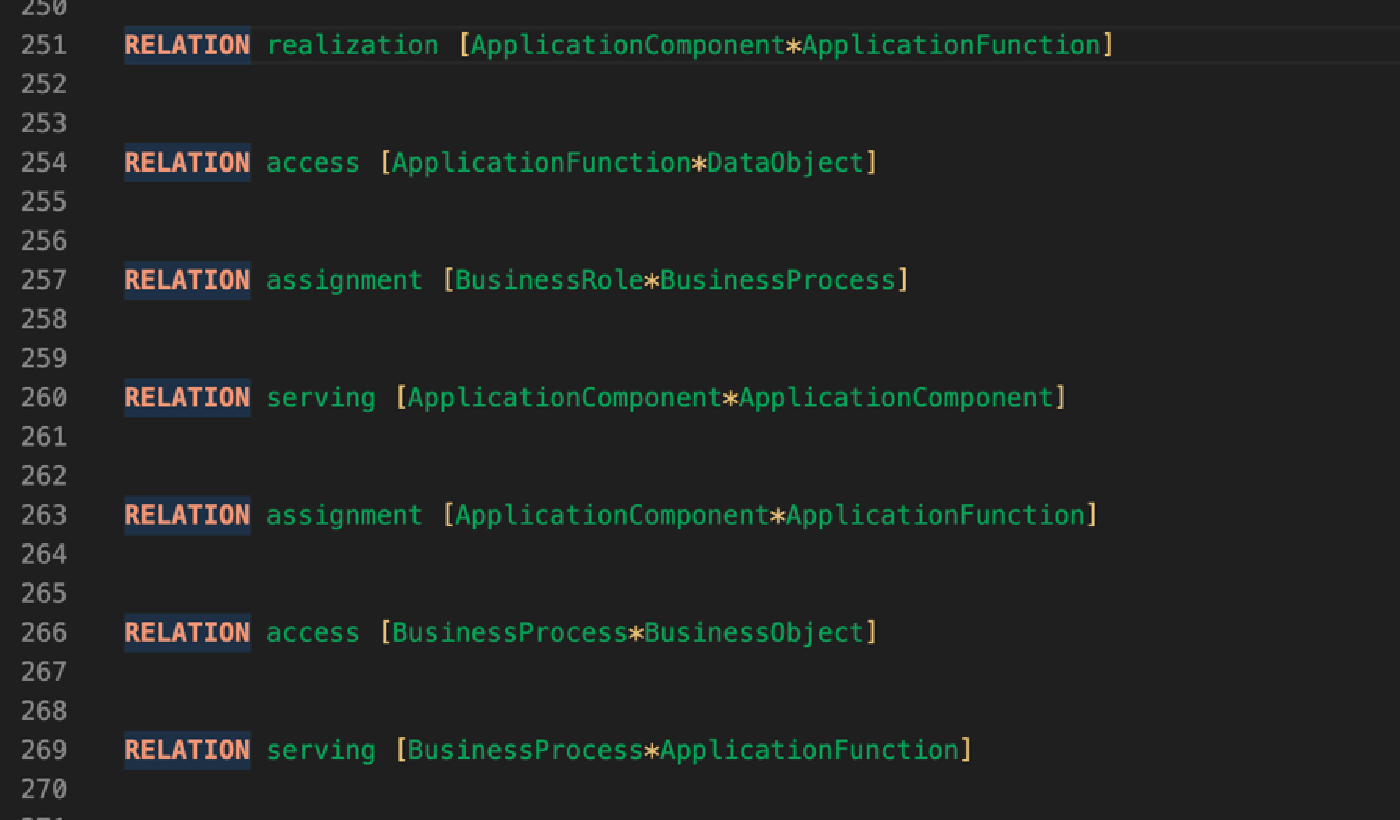
\includegraphics[clip=true, scale=0.5]{MetamodelArchiMate generated by ArchiChecker}
\caption{Metamodel fragment of ArchiMate as generated by Ampersand}
\label{meta}   % Give a unique label
\end{figure}
Generating the metamodel directly from the ArchiMate model ensures that there can be no discrepancy between the metamodel and the data that represents the ArchiMate model.
This prevents programming mistakes when matching the data from an ArchiMate model to the metamodel.

Figure~\ref{populated} shows a fragment of the internal representation of an ArchiMate model (i.e. the .archimate-file in which Archi stores its model) generated by Ampersand.
The long numbers are unique numbers representing instances of elements in ArchiMate.
\begin{figure}[hbtp]
 \centering
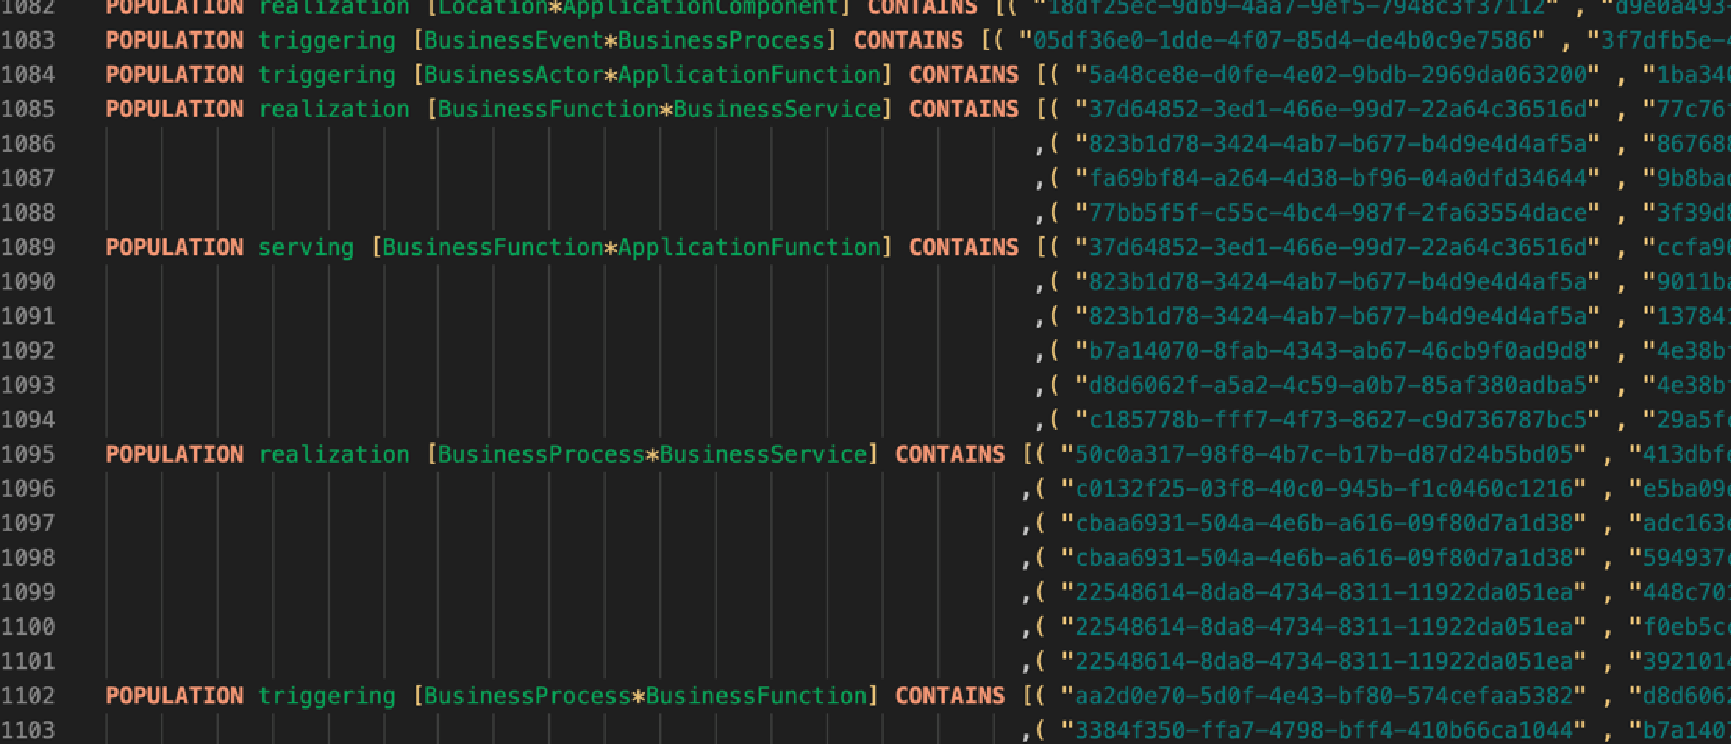
\includegraphics[clip=true, scale=0.4]{Populated model}
\caption{An internal ArchiMate representation of a model.}
\label{populated}   % Give a unique label
\end{figure}

%
\begin{figure}[hbtp]
 \centering
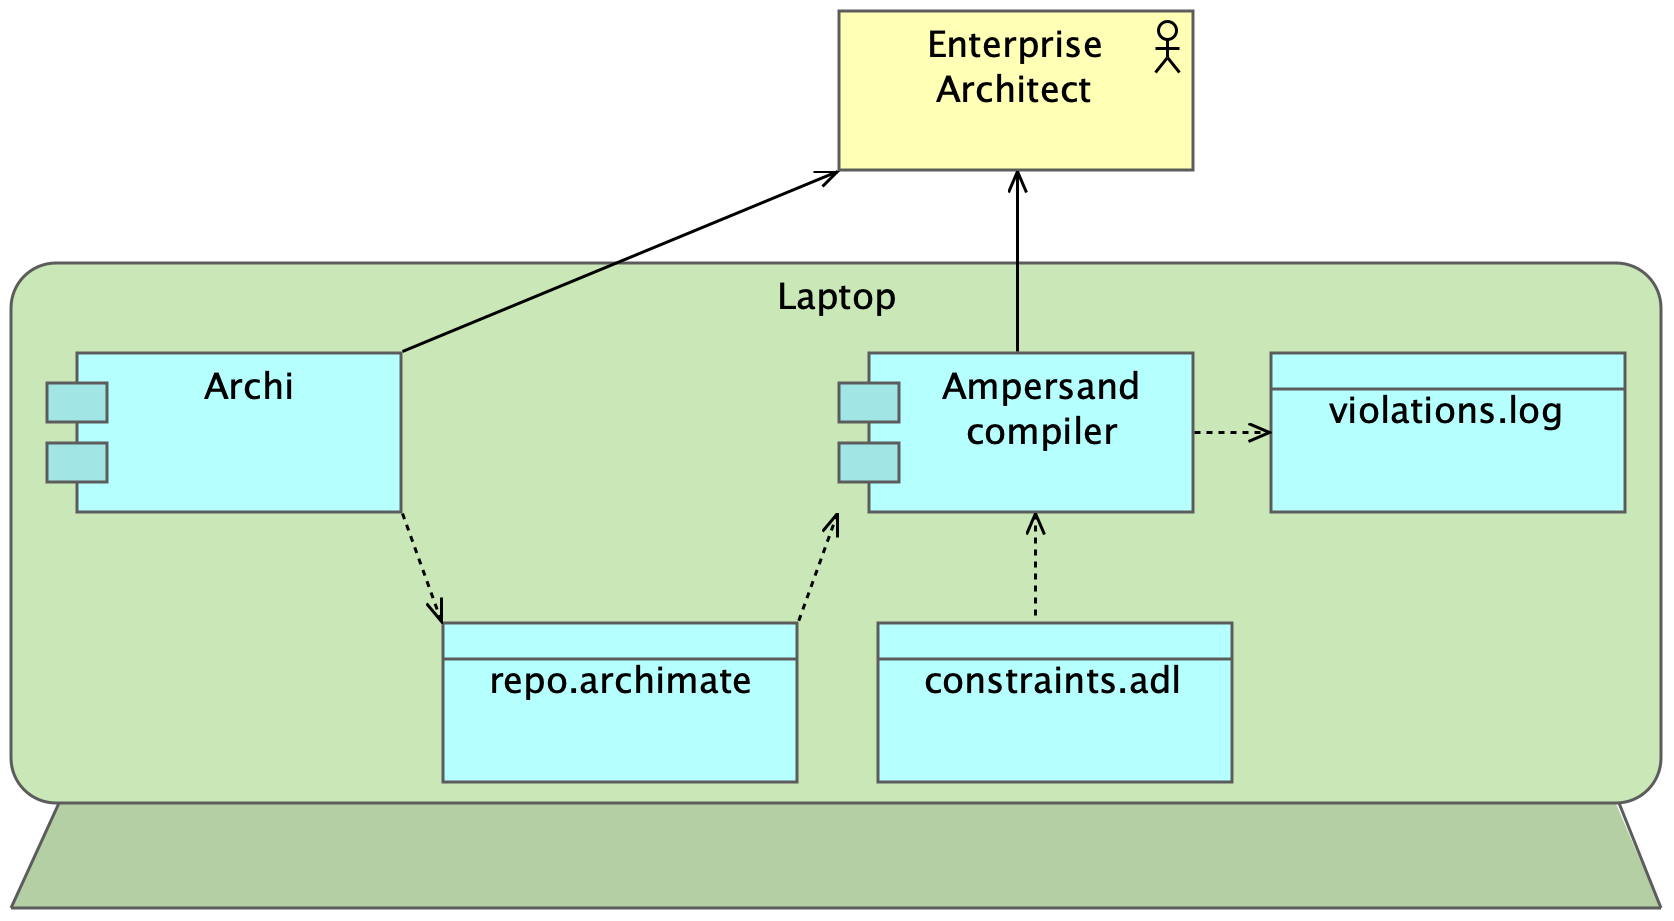
\includegraphics[clip=true, scale=0.19]{Figure4}
\caption{A toolset for an enterprise architect~\cite{iceis22}.}
\label{fig2}   % Give a unique label
\end{figure}
\begin{figure}[hbtp]
 \centering
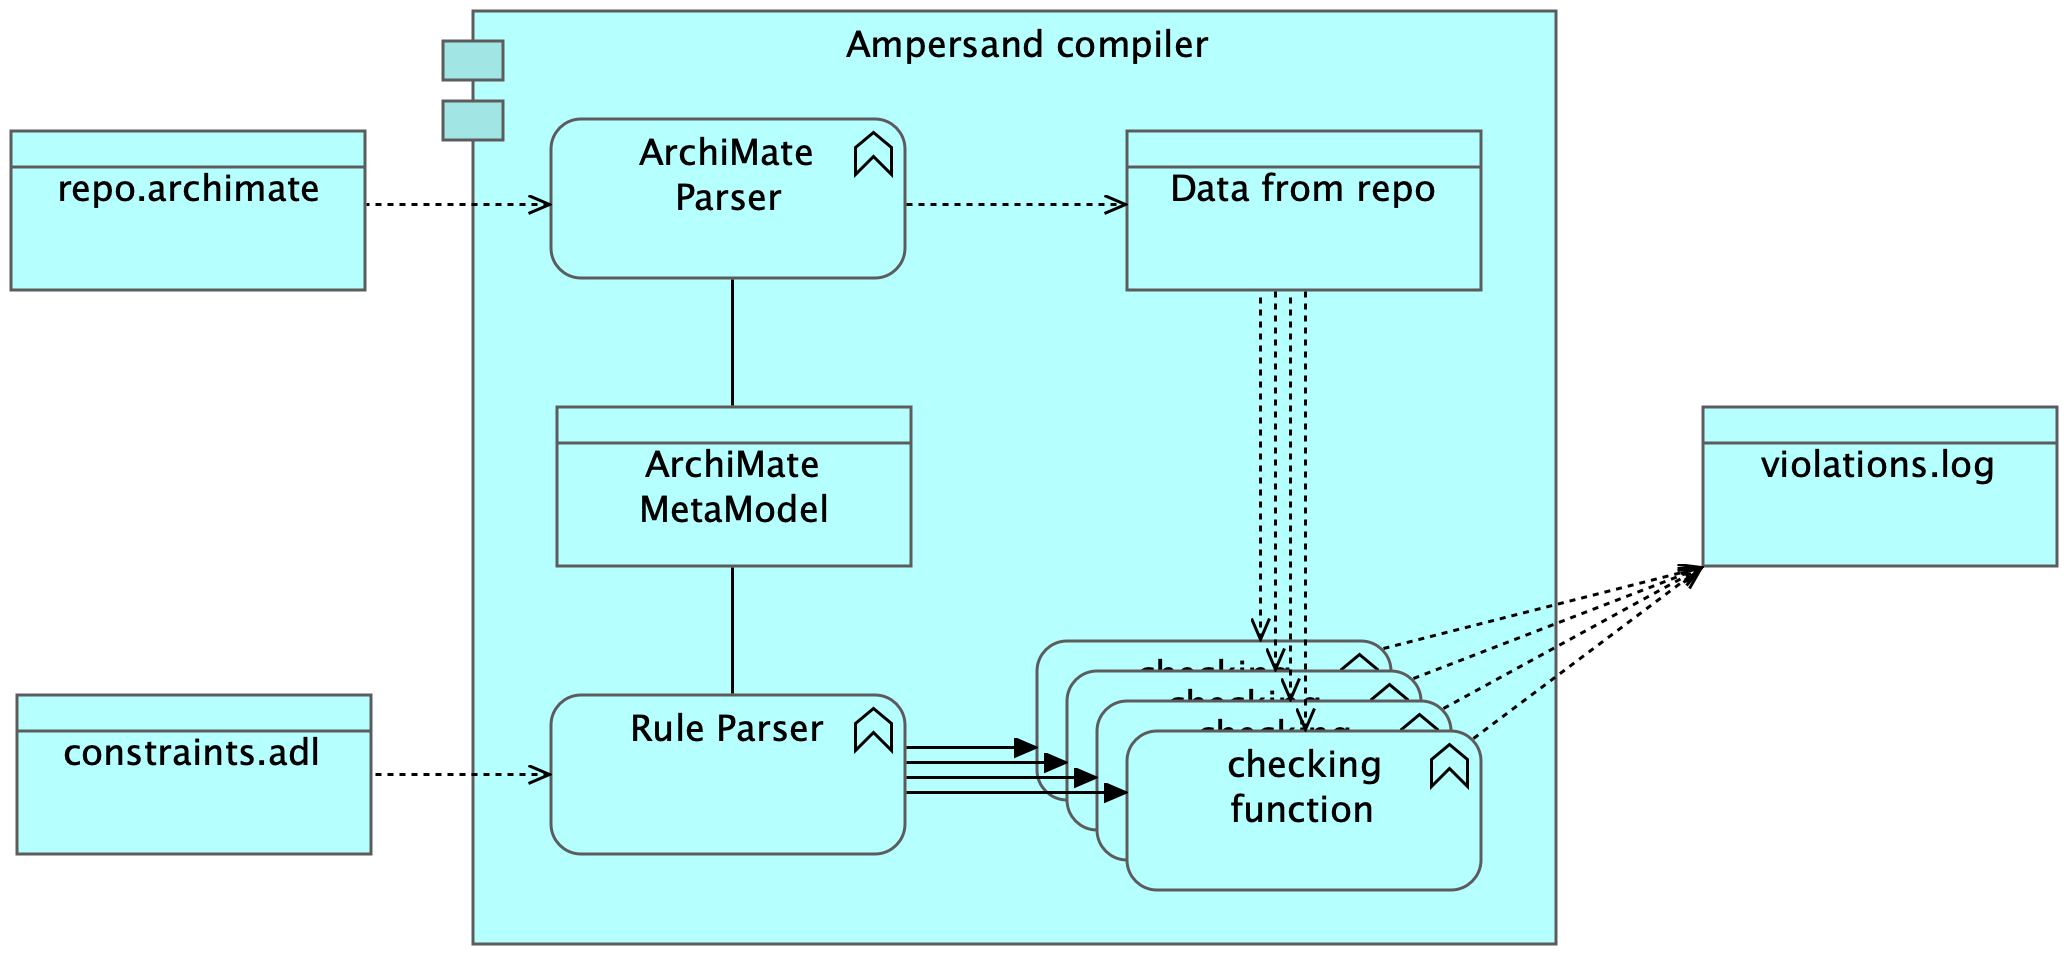
\includegraphics[clip=true, scale=0.16]{Figure5}
\caption{Under the hood of the Ampersand compiler~\cite{iceis22}.}
\label{fig3}
\end{figure}

Two tools serving the enterprise architect are shown in figure~\ref{fig2}: an ArchiMate modeling tool and the Ampersand compiler.
In figure~\ref{fig2} the file in which Archi stores an ArchiMate model is called ``repo.archimate''.
Constraints are stored in the the file called ``constraints.adl''.
The component ``Ampersand compiler'' compiles the ArchiMate model (``repo.archimate'') together with the constraints (``constraints.adl'') into a set of violations (``violations.log'').

What happens ``under the hood'' of the Ampersand compiler is illustrated in figure~\ref{fig3}.
The ArchiMate model is parsed according to the ArchiMate metamodel.
Constraints are parsed according to the same metamodel, because a constraint checker must ``know'' where to find the data to be checked.
For each constraint, a checking function is generated that can compute violations with respect to that constraint.
All violations found by the Ampersand compiler are emitted to the ``violations.log''.

So now, let us look at the constraints and the way violations of these constraints are used.

\subsection{The Making of Constraints}\label{Analyzing Models}
To gain some understanding of the internal functioning,
let us look at a small fragment of the ArchiMate metamodel, figure~\ref{meta}.
The ArchiMate metamodel consists of relations\footnote{In this paper, the word ``relation'' refers to the mathematical notion of relation and to a relation in Ampersand, which are the same.
The word ``relationship'' refers to the corresponding notion in ArchiMate.}, each of which contains pairs.
These pairs form the population of the relations in the metamodel, as illustrated in figure~\ref{populated}.
For example, the relation \verb#realization# represents a set of pairs,
each of which relates one particular Business Function to one Business Service.

Within the Ampersand compiler, the metamodel defines the relations.
The compiler ``grinds'' an ArchiMate model into pairs that populate these relations (figure~\ref{populated}).
The long numbers that constitute pairs are the internal Archi keys for instances of ArchiMate elements, relationships, and views.
After compilation, each relation contains all pairs from all views.
So, the scope of this relation is the entire ArchiMate model.

Let us consider an example of a simple modeling convention.
Suppose the architects agree that each application component must serve at least one business process.
They agree that every graphical element that is an application component in ArchiMate must serve at lease one Business Process.
In our opinion they should also agree on the relevance of this convention:
They want all application components to be used,
so they want to signal all application components that are not used.
\begin{figure}[hbtp]
\centering
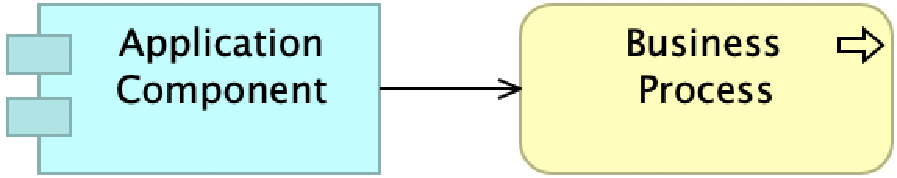
\includegraphics[clip=true, scale=0.4]{policy3}
\caption{\small Example of a modeling convention}
\label{Policy3}
\end{figure}

In Ampersand, the modeling convention is formalized into the following:
%\lstset{basicstyle=\ttfamily}
{\small
\begin{lstlisting}[frame=single, label={rulepolicy3}, caption={}]
RULE MC3
 I[ApplicationComponent] :- 
   serving ; I[BusinessProcess] ; serving~
\end{lstlisting}
}
For readers who are unfamiliar with the relation algebraic notation of Ampersand, we translate it to predicate logic:
\[\forall f \in Business\;Process \;\exists c\in Application\;Component:\; c \;serving \;f\]

Notice that every modeling convention is expressed in terms of relations that are stored in the ArchiMate tool.
If a modeling convention is formalized into a constraint, the formalization must use the relations that are defined inside the ArchiMate tool.
The Ampersand compiler harvests these relations from the .archimate-file that holds the model.

The reason to formalize in Ampersand is that ArchiMate's metamodel consists of relations.
Relation algebra is particularly suited for manipulating relations.
The language Ampersand~\cite{joosten2018relation} is a syntactically sugared version of relation algebra.
And therefore Ampersand is an obvious choice for this purpose.
So, if an enterprise architect wants to formalize modeling conventions and let the Ampersand compiler verify them, she will have to learn Ampersand.

The violations produced by a constraint are pairs,
so the set of violations may be interpreted as a relation too.
However, for practical use we are more interested in a readable form of the violation.
For this purpose the enterprise architect adds a specification to the constraint,
so the Ampersand compiler can produce readable sentences.
This is an example of a violation specification:
{\small
\begin{lstlisting}[frame=single, label={violation}, caption={}]
VIOLATION (TXT "Application component \'", TGT name, TXT "\'
 is not serving a Business process.")
\end{lstlisting}
}

Using this specification, the Ampersand compiler logs the found violations:
{\small
\begin{lstlisting}[frame=single, label={log}, caption={}]
There are 12 violations of RULE "MC3":
Application Component 'IBIS'
    is not serving a Business Process.
Application Component 'Central application (MKB)'
    is not serving a Business Process.
       ...
\end{lstlisting}
}
We have truncated these violations for brevity's sake.
There are twelve application components that do not serve any business process.
Now, architects can go back to their ArchiMate model and fix them.
They can either relate the violating application components to the business processes they serve, or remove them because they serve no purpose.
And if none of these alternatives is viable, they might even rethink the modeling convention itself.
In this way, detecting violations helps to improve Archimate models.
If the constraint gives no violations, an architect can safely claim that every application component serves a business process.
She can then also claim that this has been verified by a computer.

\section{A Case Study: Host Families}\label{host families}
To illustrate what semantics can do for an ArchiMate model, we have built a case study.
It is derived from an actual real-world situation, but it has been harnessed a little for the sake of presentation.
In this paper we only show the relevant diagrams (called ``Views'' by ArchiMate) out of a larger set of diagrams.
The hostfamily application is an information system that supports the placement of international trainees with host families throughout the country.
Since the placement is typically from 2 months to a year, some trainees may even bring their family.
To ensure the success of each placement, each situation asks for careful matching process of trainees with host families.
This matching is done by a volunteer organization, whereas responsibility of the placement lies with the national trainee programme organization.
Some two dozen factors are matched (by hand), varying from languages spoken, to disabilities, allergies, and many more.
Even though te business process has its complications, the information system to support it is rather straightforward.
Yet, the use of the hostfamily application by various stakeholders calls for a careful design.

The business process is shown in figure~\ref{fig: Business Process}.
\begin{figure}[hbtp]
 \centering
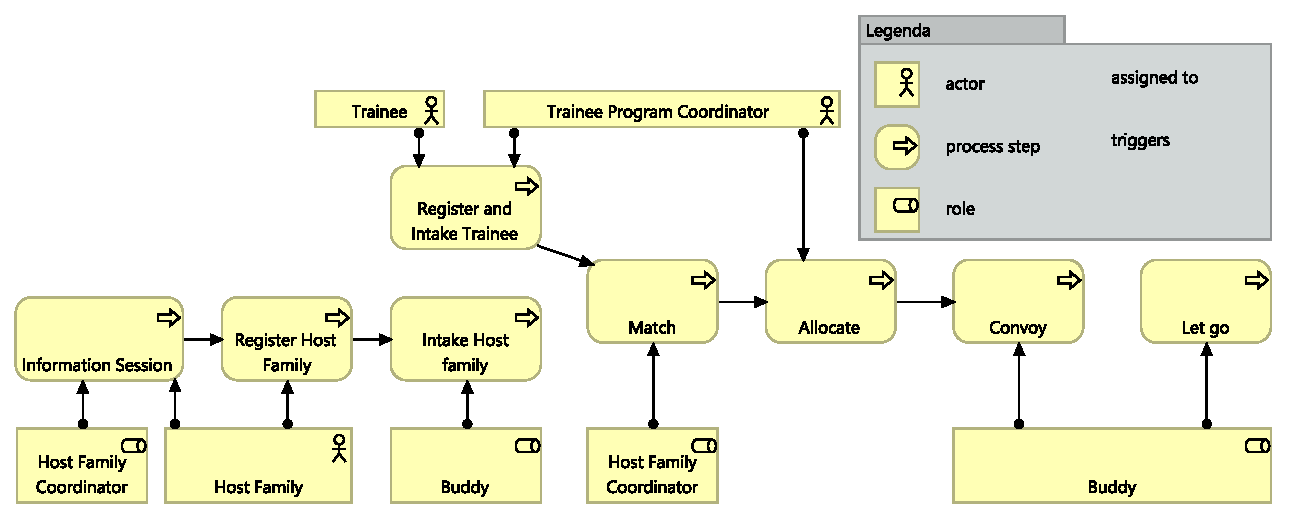
\includegraphics[clip=true, scale=0.5]{Business Process with legend.pdf}
\caption{Matching and allocating trainees with host families}
\label{fig: Business Process}
\end{figure}
The organization that recruits host families is a volunteer organization that is entirely separate from the organization that sends out the trainees.
Both organizations do their own intake, so there is ample knowledge about the trainees and about the host families to get a good match.
The volunteer organization assigns buddies (also volunteers) to convoy the host families during the placement.
A buddy provides a familiar face, a phone number to call, a listening ear, and practical assistance for any issues that might occur.
The match is made by a coordinator, who spends (on average) 4 hours to find the right host family and make all the final arrangements.
Typically, it takes just a few days for a trainee to apply for a host family until the moment of actual placement.
For this reason, the host family organization holds a larger number of host families in a register.

The hostfamily application is used by a trainee program coordinator, a host family coordinator and buddies.
The only thing a host family and a trainee can do in the system is register themselves.
Parts of the software runs on client nodes in an office, which are virtual PC's.
Parts of the software also runs on mobile devices.
For the sake of this presentation, we distinguish only two environments: Mobile and Client nodes.
The actual registration of data is done in the cloud, making all services essentially stateless.
So if anything happens with client hardware, the data is still safe.

\begin{figure}[hbtp]
 \centering
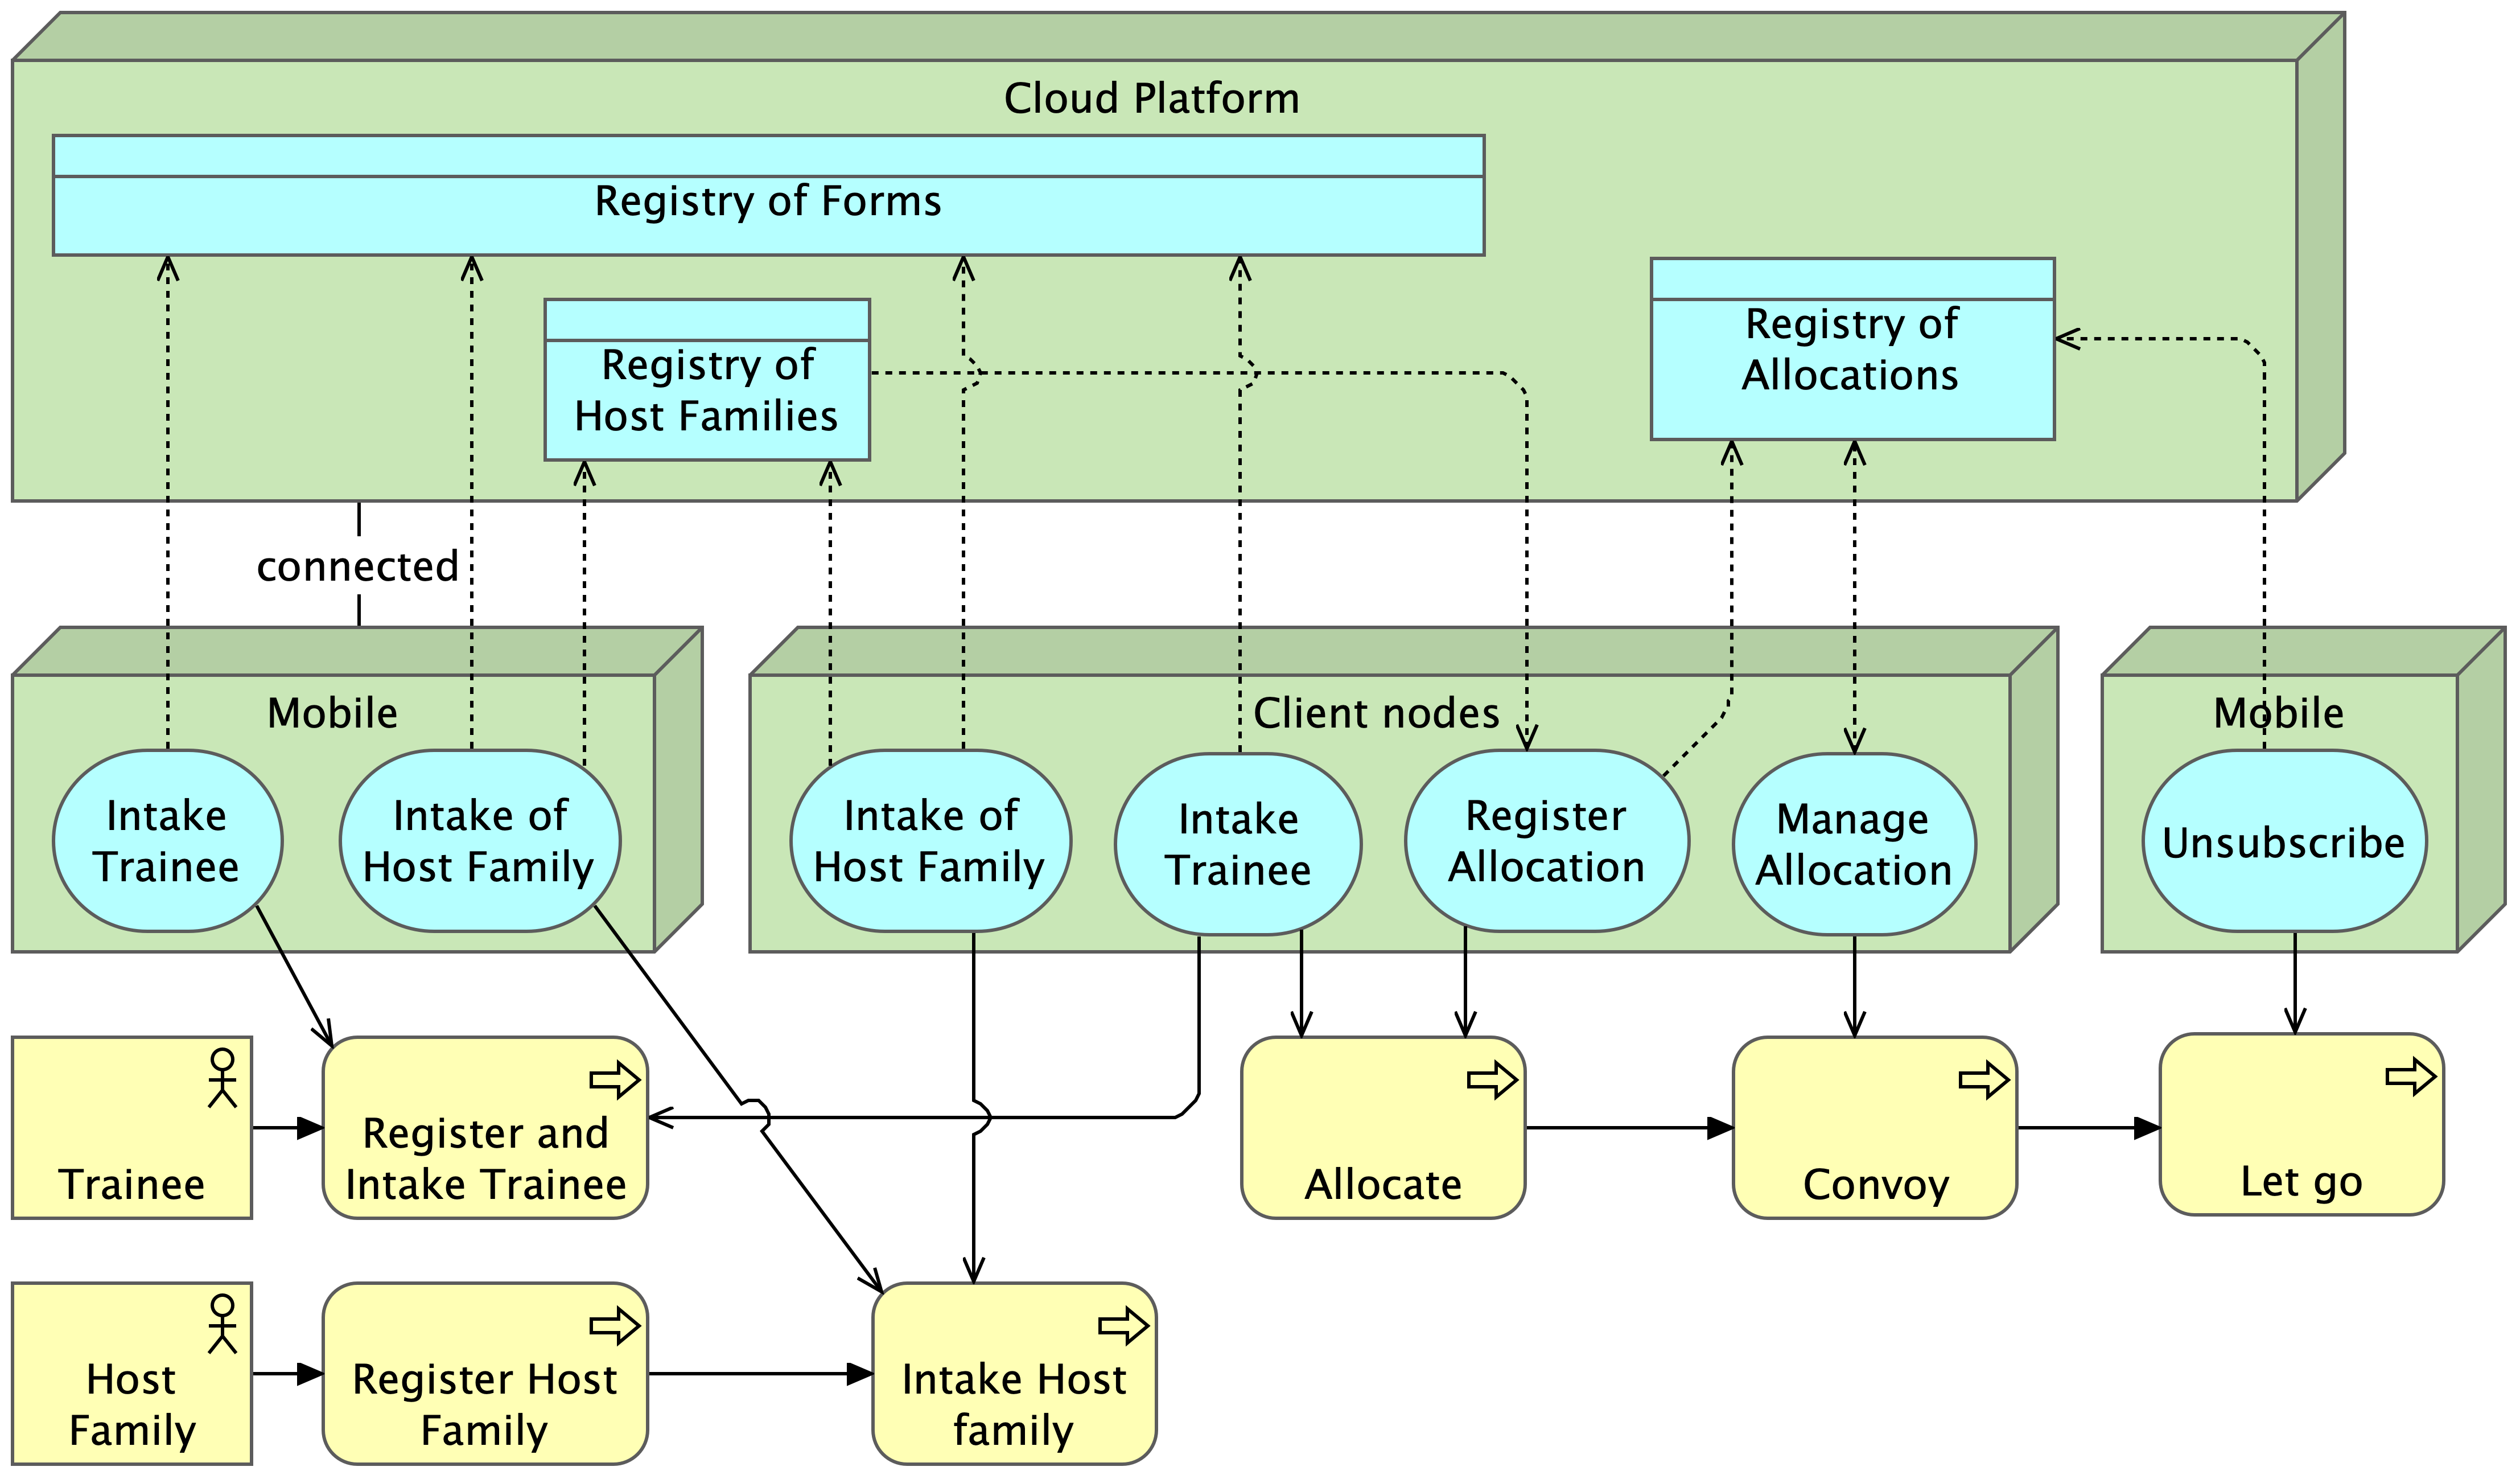
\includegraphics[clip=true, scale=0.07]{Services voor Uitvoering.png}
\caption{Business processes aligned with microservices}
\label{fig: Alignment of services with business processes}
\end{figure}

Figure~\ref{fig: Alignment of services with business processes} shows which application services are serving which business processes.
We have used ArchiMate's application services to model microservices of the hostfamily application.
It also shows on which platforms which services are running.

In the previous section we saw that architects are not always the best audience to elicit their own modeling conventions.
In this case study, the authors have suggested the modeling conventions themselves.
Suggestions were based on the author's knowledge of architecture in general and the business process at hand.
Rather than ask architects from the business, we talked to users and other business stakeholders.
Modeling conventions were crafted after carefully listening and discussing.
This has the added advantage the we can use the method also in smaller organizations that do not have the architectural expertise,
as was the case in this situation.

Each of the following five sections applies one constraint to the ArchiMate model.
Each modeling convention is represented by a constraint for a purpose,
which we explain with the constraint.

\subsection{Modeling Convention 1}
The first modeling convention is that every business process must be served by at most one microservice.

A visualization of the convention is shown in figure~\ref{MC1}.

\begin{figure}[hbtp]
\centering
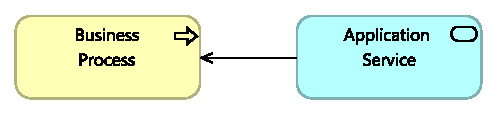
\includegraphics[clip=true, scale=0.7]{MC1}
\caption{\small{Every business process must be served by at most one microservice.}}
\label{MC1}
\end{figure}

{\small
\begin{lstlisting}[frame=single, label={mc1}, caption={Every business process must be served by at most one microservice.}]
RULE Maintainable microservices :
   I[BusinessProcess] :- -(serving~;
   -I[ApplicationService];serving)
VIOLATION ( TXT "Business Process "
          , SRC name
          , TXT " is served by multiple 
              microservices: "
          , SRC serving~;name)
\end{lstlisting}
}
Again, for the sake of readers less familiar with relation algebra, we give the constraint in predicate logic:
\[\begin{array}{rcl}
   \multicolumn{3}{l}{\forall p \in Business\;Process, \;\forall a,b\in Application Service:}\\
   p \;serving \;a\ \wedge\ p \;serving \;b&\Rightarrow&a\not =b
\end{array}\]

The Ampersand compiler responds with:

{\small
\begin{verbatim}

There is one violation of RULE "Maintainable microservices":
Business Process "Allocate" is served by multiple microservices:
  {"Register Allocation", "Intake Trainee"}

\end{verbatim}
}

Indeed, in figure~\ref{fig: Alignment of services with business processes},
we can see that the constraint has spotted the misalignment.
Removing the serving relation between application service ``Intake Trainee'' and business process ``Allocate'' solves the problem.

Note that the person who models the modeling convention (syntax: \verb#RULE#) will also specify which message is produced for each violation (syntax: \verb#VIOLATION#).

\subsection{Modeling Convention 2}
The second modeling convention is that every business process should be served by a microservice.
The purpose is to ensure that every step is supported by a service in the hostfamily application, unless there is a conscious decision to the contrary.
This helps an architecture team to spot omissions.
In terms of visualization we can reuse figure~\ref{MC1}, even though this second modeling convention differs from the first one.
It resembles the example in section~\ref{Analyzing Models}, but there too is a difference.
This constraint talks about application services and the other one about application components.
For ArchiMate these are different types of elements, so they require separate constraints\footnote{unless application components and application services are defined to be synonym in Ampersand. Ampersand can deal with that.}.

{\small
\begin{lstlisting}[frame=single, label={mc2}, caption={}]
RULE Coverage:
   I[BusinessProcess] :- serving~;
   I[ApplicationService];serving
VIOLATION ( TXT "Business Process "
          , SRC name
          , TXT " is not served by any 
          microservice.")
\end{lstlisting}
}

The Ampersand compiler responds with:

{\small
\begin{verbatim}

There are 4 violations of RULE Coverage:
Business Process "Information Session" is not served by any
     microservice.
Business Process "Match" is not served by any microservice.
Business Process "Register Host Family" is not served by any
     microservice.
Business Process "Register and Intake Trainee" is not served by any
     microservice.

\end{verbatim}
}

Looking at figure~\ref{fig: Alignment of services with business processes},
notice that business processes ``Information Session'' and ``Match'' do not occur in figure~\ref{fig: Alignment of services with business processes}.
However, they do occur in figure~\ref{fig: Business Process} and Ampersand computes the violations throughout the entire model (accross all views).

From these violations, the design team can draw its conclusions.
Let us assume they want to include the missing application services into the model,
except for the business process ``Information Session'' because it requires no support.

\subsection{Modeling Convention 3}
The third modeling convention is to show that semantics can also involve infrastructure,
as ArchiMate caters for infrastructural modeling as well as for modeling of applications and business.
The third modeling convention says that if you want to access a data object on another platform, the infrastructure needs to be in place.
Or stated more precisely:
If an application service, which is realized by a node or device $n$, wants to access a data object $d$,
device $n$ must be connected to the node or device in which $d$ resides.
The purpose of this modeling convention is to ensure that the required connections are made explicit in the ArchiMate model.

\begin{figure}[hbtp]
\centering
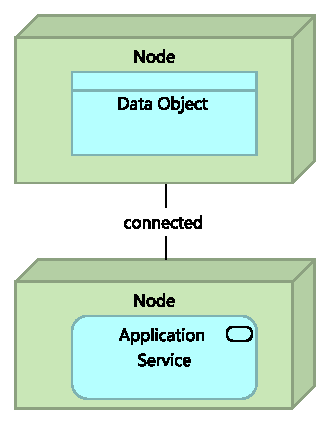
\includegraphics[clip=true, scale=0.7]{MC3}
\caption{\small{If an application service, which is realized by a node or device $n$, wants to access a data object $d$,
device $n$ must be connected to the node or device in which $d$ resides.}}
\label{MC3}
\end{figure}

{\small
\begin{lstlisting}[frame=single, label={mc3}, caption={}]
CLASSIFY Device IS Node
RULE Infra1:
   realization;access :- (I\/connected\/connected~);access
VIOLATION ( TXT "ApplicationService "
          , SRC realization;name
          , TXT " on node "
          , SRC name
          , TXT " cannot access data object: "
          , TGT name)
\end{lstlisting}
}

The Ampersand compiler responds with:

{\small
\begin{verbatim}

There are 3 violations of RULE Infra1:
ApplicationService { "Intake of Host Family", "Manage Allocation"
                   , "Register Allocation", "Intake Trainee"}
on node "Client nodes" 
cannot access data object: "Registry of Allocations"

ApplicationService { "Intake of Host Family", "Manage Allocation"
                   , "Register Allocation", "Intake Trainee"}
on node "Client nodes" 
cannot access data object: "Registry of Host Families"

ApplicationService { "Intake of Host Family", "Manage Allocation"
                   , "Register Allocation", "Intake Trainee"}
on node "Client nodes" 
cannot access data object: "Registry of Forms"

\end{verbatim}
}
In figure~\ref{fig: Alignment of services with business processes},
we see that precisely all services that run on the Client nodes cannot communicate with the cloud.
This implies that we need a connection between the Client nodes and the Cloud platform.
After we add an association called ``connected'' between the two, no violations remain and the problem is solved (Figure~\ref{fig: Adapted service alignment}).

Notice that this modeling convention is useful only in situations where infrastructure is an issue.
For example, an application that is distributed over different platforms may benefit from an explicit modeling of infrastructure.
So, the person proposing a modeling convention must be able to judge whether modeling the infrastructure has value for his architecture team.

\subsection{Modeling Convention 4}\label{Modeling Convention 4}
The fourth modeling convention is:
If a business role or a business actor is assigned to two subsequent process steps that are being serviced,
these steps must be realized by application services on the same node or device.

The purpose is to ensure that a user can finish subsequent process steps without switching devices,
which makes the hostfamily application more user-friendly.

{\small
\begin{lstlisting}[frame=single, label={mc4}, caption={}]
RULE SubsequentSteps:
   triggering[BusinessProcess]/\serving~;V;
   serving /\ assignment~;assignment
    :- serving~;realization~;I[Node];realization;serving
VIOLATION ( TXT "Business Role "
          , SRC assignment~;name
          , TXT " wishes to perform steps "
          , SRC name
          , TXT " and "
          , TGT name
          , TXT " on the same device.")
\end{lstlisting}
}

The Ampersand compiler responds with:

{\small
\begin{verbatim}

There is one violation of RULE SubsequentSteps:
Business Role "Buddy" wishes to perform steps "Convoy" and "Let go"
on the same device.

\end{verbatim}
}
Comparing this message with figure~\ref{fig: Alignment of services with business processes},
we notice that the microservice ``Unsubscribe'' should run on mobile devices as well as on client nodes.

Figure~\ref{fig: Adapted service alignment} shows the result of applying the proposed changes in ArchiMate for all four modeling conventions discussed up to this point:
\begin{figure}[hbtp]
  \centering
  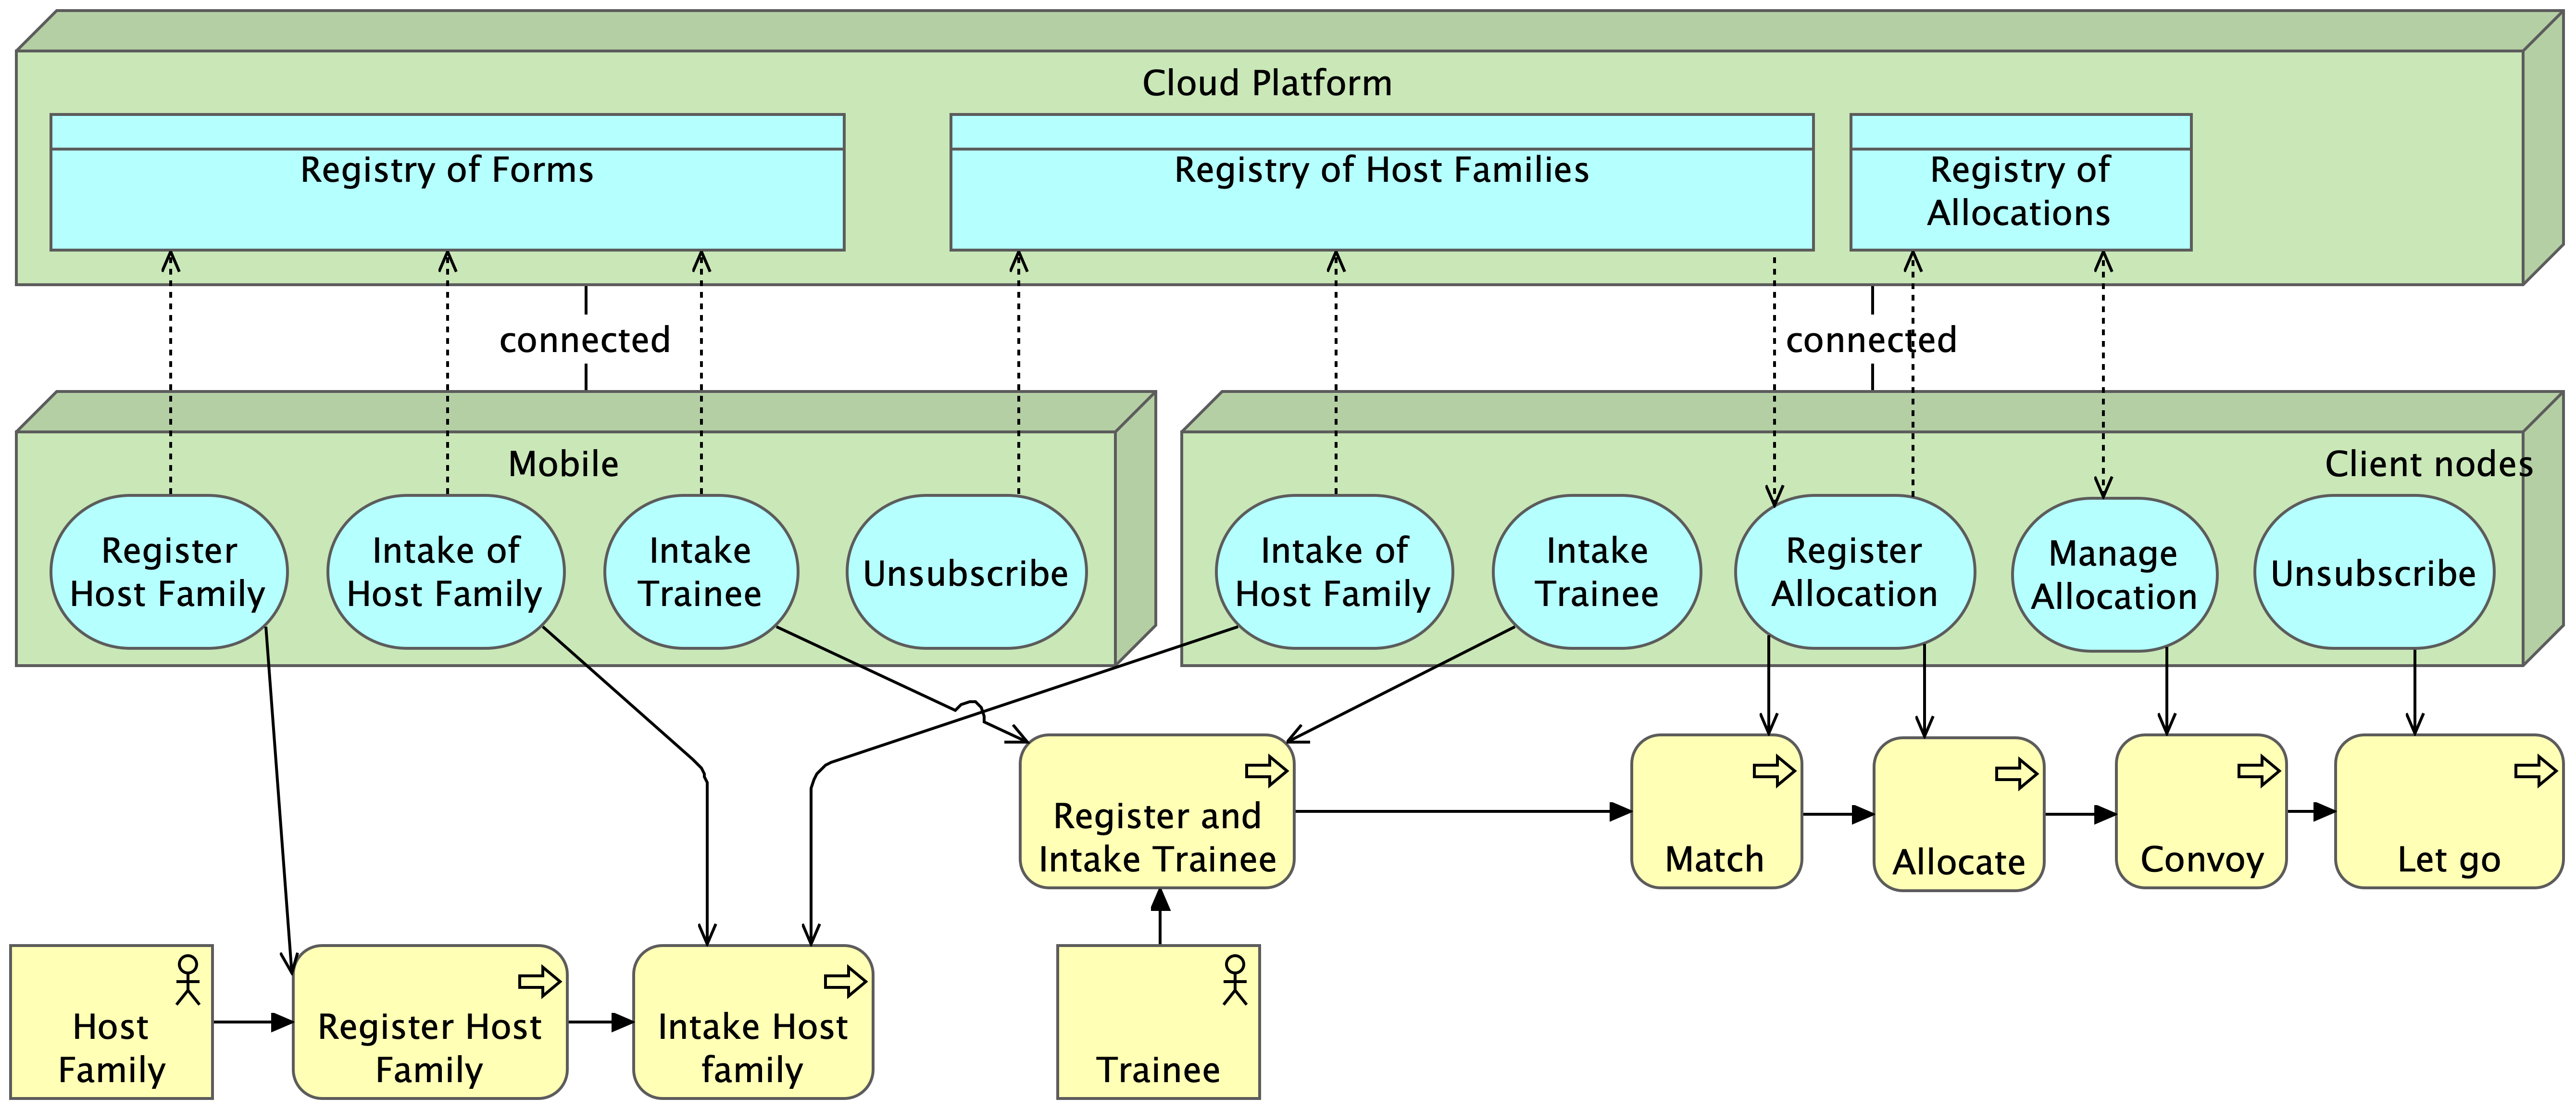
\includegraphics[clip=true, scale=0.06]{Services na correcties.png}
  \caption{Business processes aligned with application services}
  \label{fig: Adapted service alignment}
\end{figure}

Having checked 4 modeling conventions and made changes accordingly, we can now make the following claims:
\begin{enumerate}
    \item Every business process in the ArchiMate model is being served by at most one microservice.
    \item Every business process except ``Information Session'' is being served by an application service.
    \item Every application service in the ArchiMate model is connected to the registries from which it takes data objects.
    \item Every person can perform subsequent steps in the process on the same device.
\end{enumerate}
We can also state that these claims have been formally checked and verified by the Ampersand compiler,
so now it is up to the builders of the hostfamily application to make a faithful implementation of the design.

When checking the new model (figure~\ref{fig: Adapted service alignment}), there is only violation left:
Business process ``Information Sessions'' is not served by any application service.
This is precisely what the architects want.

A careful inspection of figure~\ref{fig: Adapted service alignment} reveals that
the application service ``Unsubscribe'' on the Mobile platform has no serving relationship with business process ``Let go",
whereas the same application service on the Client nodes does.
In this situation, the architect has made clever use of ArchiMates aliasing mechanism;
he has made both application service ``Unsubscribe'' into aliases of each other.
They are in fact one and the same application service.
So a relationship with one of these shapes counts for both.
In the same picture, both application services "Intake Trainee" from Client nodes and Mobile do have a serving relationship to "Register and Intake Trainee",
even though these application services are aliases of the same ArchiMate element.
So the modeler has made a different choice here.
In ArchiMate, this may be confusing.
Two shapes of the same type with the same name may be the same (i.e. have the same internal ArchiMate identifier)
but they may also be different (i.e. have different internal ArchiMate identifiers).
For this reason we advise architects to ensure that they identify all shapes with the same name and type as the same ArchiMate object.
Ampersand can work with both alternatives, but the results of constraint verification may be somewhat unpredictable when the architect
adopts makes no clear choice.
The choice we advise has the attractive property that fewer relationships need to be drawn, which saves on clutter in the diagrams.

\subsection{Modeling Convention 5}
So what about further refinements? Does a refinement involve changing earlier constraints?
For reasons of maintainability and scalability, we would like to refine the model by adding constraints rather than revising existing constraints.
In this fifth modeling convention we will do such a refinement by just adding a constraint.
So let us refine the connectivity from modeling convention 3.

The reader might already have noticed that the association called ``connected'' is somewhat gratuitous.
Just adding a link does not say much about the infrastructure that is needed between the different nodes.
At least, we should model which networks are used to connect these nodes.
For this reason we add a constraint that says that every connection requires that there is a network to connect both ends.
Since this modeling convention only constrains the relationship ``connected'',
none of the existing constraints is affected.
In this way we have added detail about infrastructure (or any other subject) incrementally.

{\small
\begin{lstlisting}[frame=single, label={mc5}, caption={}]
RULE "Network Connections": connected :- connects;connects~
VIOLATION ( TXT "Node "
          , SRC name
          , TXT " has no network to connect with node "
          , TGT name
          , TXT ".\n   To resolve this, please use 
                       an association "
          , TXT "connect[Node*Network] to connect  "
          , TXT " these nodes to the same network.")
\end{lstlisting}
}

The Ampersand compiler responds with:

{\small
\begin{verbatim}

There are 2 violations of RULE "Network Connections":
Node "Cloud Platform" has no network to connect with node "Mobile".
  To resolve this, please use an associations connect[Node*Network]
  to connect these nodes to the same network.
Node "Client nodes" has no network to connect with node 
     "Cloud Platform".
  To resolve this, please use an associations connect[Node*Network]
  to connect these nodes to the same network.

\end{verbatim}
}

To describe the communication in terms of networks, we can make a new ArchiMate view:
\begin{figure}[hbtp]
   \centering
   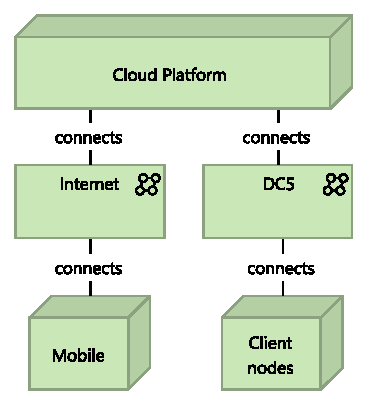
\includegraphics[clip=true, scale=0.9]{Network connections.pdf}
   \caption{Adding networks to describe the communication}
   \label{fig: Network connections}
\end{figure}
After adding this view, the Ampersand compiler is satisfied.
The addition of this extra modeling convention now means that we can make an extra claim:
\begin{enumerate}
    \item Every connection in the ArchiMate model has a network assigned to it.
\end{enumerate}

\begin{figure}[hbtp]
 \centering
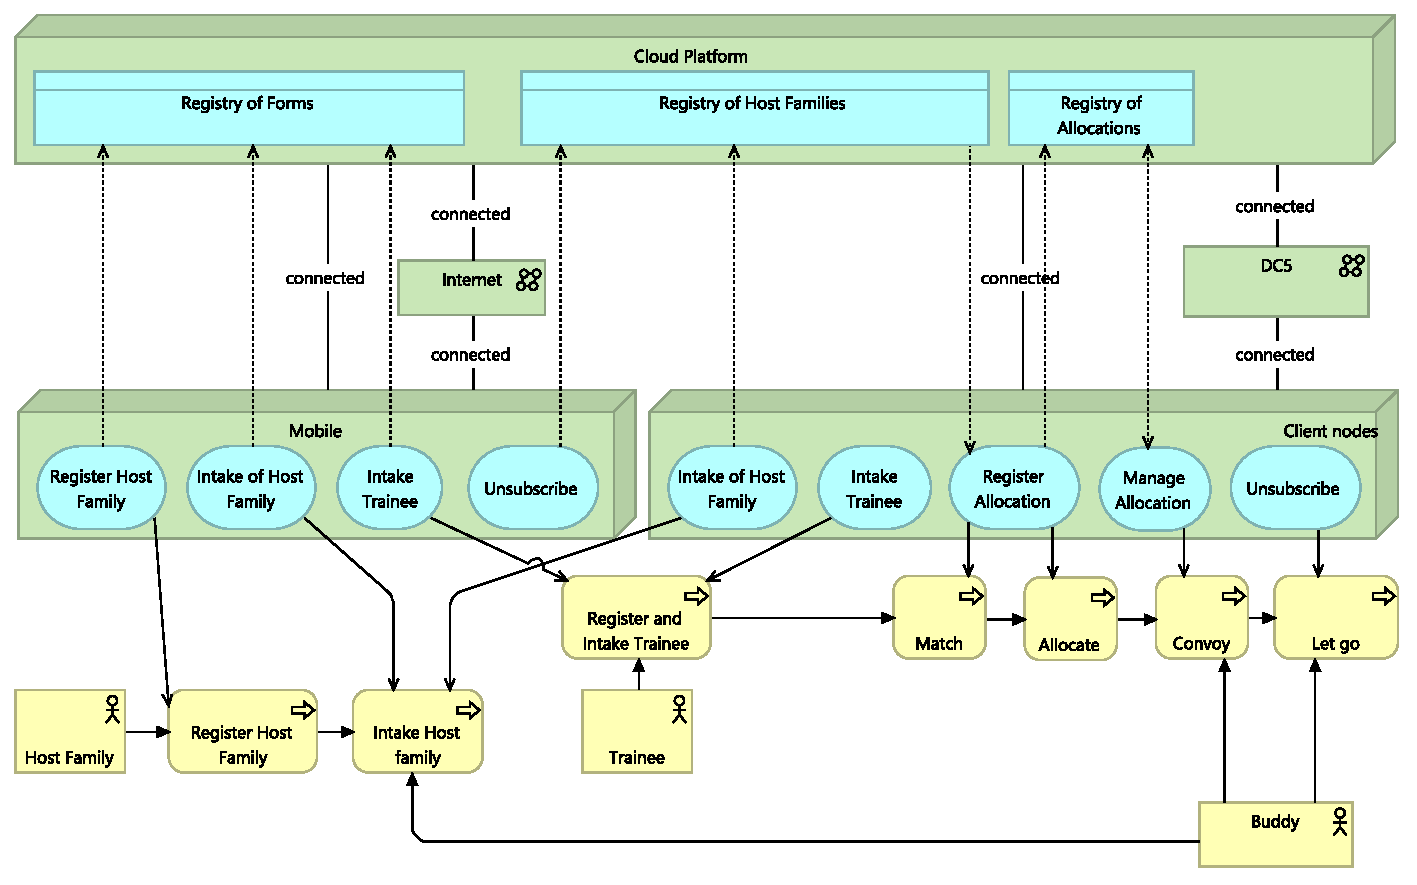
\includegraphics[clip=true, scale=0.48]{Services 3.pdf}
\caption{Business processes aligned with application services}
\label{fig: Alignment of services with business processes 3}
\end{figure}

\section{Reflection and Lessons Learned}\label{reflection}
During the first study we did in the quest for an ArchiChecker~\cite{filetenterprise},
we believed that checking constraints could help us to rate the quality of ArchiMate models in a reproducible manner.
In the study we did at UMCU~\cite{iceis22}, we learned that our method would never do that.
The reason is that the constraints are imposed directly on an ArchiMate model, so the best we can do is verify modeling conventions of a team.
Fortunately, this is quite useful because every team has different concerns.
So the team can make an effort to translate their own concerns to modeling conventions (informally)
and then verify the corresponding constraints (that are formal) automatically.

Other revelations followed from the discussions with architects at UMCU.
At the outset of this project we hoped that architects who use ArchiMate could easily tell us about the modeling conventions they adhere to.
However, we found that only few modeling conventions were in place.
Experience with other organizations gives us no reason to believe that UMCU is exceptional in this respect.
So, we made architects think about modeling conventions and come up with suggestions,
to see whether we could formalize them.
All but one of the modeling conventions they came up with turned out to be representable as multiplicity constraints.
In complexity, that is comparable to the example in section~\ref{Analyzing Models}.
However, relation algebra can express way more than multiplicity constraints only\footnote{Theoretically, predicate logic can express even more than relation algebra, but in practice this rarely occurs.}, so we felt there was much more potential.
However, the architects did not come up with more complex constraints.
Even worse, these architects did not think the violations of their own modeling conventions were very meaningful.
They had other concerns to attend.
In retrospect, we had failed to pay attention to the relevance of modeling conventions.
From this study, we learned to focus on modeling conventions that are relevant.
It is imperative to know the concerns of stakeholders and to discuss in detail (with examples) why modeling conventions are relevant or not.

Formalization is not the issue here.
Surely, constraints set up by newbees may not represent the intended modeling conventions accurately.
But this can be fixed by ensuring that one of the architects is proficient in Ampersand.
The real issue is to come up with modeling conventions that add value to the architects.
Our case study (sct.~\ref{host families}) demonstrates that violations can be used to fix and improve ArchiMate models.
So that is the kind of relevance one must focus on in discussions and workshops.
The toolset can then help to formulate relevant modeling conventions accurately.
We have also noticed that such discussions raise the professional level of the team,
because because of the scrutiny every modeling convention receives.

Therefore we propose a cyclic approach with periodic session (e.g. 6 times a year) where architects reflect on their set of modeling conventions,
on the violations harvested with them, and produce periodic updates of the constraints to keep up with the changing demands of their environment.
This cycle serves multiple purposes:
\begin{itemize}
   \item it ensures the value of modeling conventions as the business changes;
   \item it raises the professionalism of the architecture team due to continuous reflection;
   \item it yields statements about the architecture that have been verified automatically.
\end{itemize}

It is not a good idea to ask architects to come up with ideas.
Much better is to ask them about their immediate concerns and to trace how this is reflected in their models.

The actor in such a scenario is an experienced architect who has acquired the skills to use the Ampersand compiler, especially the Ampersand language.
He or she can elicit concerns and propose modeling conventions, after trying them out first.
Experience in architecture is also needed to understand how architectural models are being used,
which types of modeling defects occur,
and which hints are useful to other architects in the group.
After trying his proposals on actual ArchiMate models, he can propose and demonstrate the constraints to his peers.
The discussion that follows should be steered in the direction of fewer constraints and more relevant constraints.

\section{Conclusions and Future Work}\label{conclusion}
There are several conclusions to be drawn from this work.
Since this case study investigates the use of modeling conventions, the conclusions are methodological in nature.

We found that enhancing ArchiMate models with semantics is not very common (yet).
However, many authors feel the need to do so (and so do we).
Apparently, this way of working with ArchiMate is still in its infancy.

The most obvious takeaway of our case study is that proposing a modeling convention works better than asking architects for suggestions.
The good news about it is that this can stimulate architects to fix or improve their models.
The bad news is that this requires the architectural skill to identify relevant modeling conventions and the formal skill to use the toolset.

Adding semantic constraints can benefit other aspects of the design than ArchiMate supports,
as is illustrated by modeling convention 4 (sct.~\ref{Modeling Convention 4}).
The modeling convention is essentially about one aspect of usability, which is not contained in ArchiMate itself.
For ArchiMate has no built-in modeling elements nor relations for usability.
This illustrates the value added by taking constraints to the level of semantics.

Another lesson is to focus on relevance.
A modeling convention is useful only if it serves a clear purpose and that purpose is deemed useful by its audience.
Enhancing ArchiMate with constraints is an effort that can easily draw the focus to other things than relevance,
making this into an academic exercise that lacks practical value.
So we need to stress this aspect in our methods.

Enhancing ArchiMate models with semantic constraints benefits architects with a way to verify their own modeling conventions.
It can also benefit their business, because an ArchiMate model can have useful properties that are verified.
This may well have consequences for the approval process, because a business can demand specific claims that address practical business concerns.
Architects can report about conformance to or violation of policies in the enterprise, once they are formalized.

Experimenting with our approach, we have found that a business policy and the corresponding constraint cannot be understood 
without understanding the goal of the Enterprise Model in hand and the goal of the business policy in it.
The method and tooling presented in this paper can be seen as a part of Enterprise modeling approach that includes goal modeling.
We are working on an approach for consistent modeling in ArchiMate that includes goal models 
refined to requirements and associated with policies and constraints within each enterprise multi-view model~\cite{severin2022}.
We believe that the applicability of constraints associated with a goal model is easier to understand,
making it easier to decide what to do with constraint violations.

\backmatter

%\bmhead{Acknowledgments}

\section*{Declarations}
For the purpose of full disclosure, the authors declare the following:

\begin{itemize}
\item This research was funded in full by the Open University of the Netherlands.
\item Neither author has any conflicting interest, nor competing interest, w.r.t. this work.
\item Ethics approval has not been sought because ethical dillemma's in this work were too small.
\item This work has been performed with participation of the UMCU in an earlier paper.
Other than that, the only participating organizations are the employers of the authors: Open University of the Netherlands and Ordina.
\item The UMCU has consented to publishing its contribution to the ArchiChecker project.
\item The data and materials and source code of this work can be found on Github (add reference)
\item Both authors have contributed equally to writing this paper. Coding has been done by Stef Joosten.
\end{itemize}


%%===================================================%%
%% For presentation purpose, we have included        %%
%% \bigskip command. please ignore this.             %%
%%===================================================%%
%\bigskip
%\begin{flushleft}%
%Editorial Policies for:

%\bigskip\noindent
%Springer journals and proceedings: \url{https://www.springer.com/gp/editorial-policies}


%\begin{appendices}

%\section{Section title of first appendix}\label{secA1}



%\end{appendices}

%%===========================================================================================%%
%% If you are submitting to one of the Nature Portfolio journals, using the eJP submission   %%
%% system, please include the references within the manuscript file itself. You may do this  %%
%% by copying the reference list from your .bbl file, paste it into the main manuscript .tex %%
%% file, and delete the associated \verb+\bibliography+ commands.                            %%
%%===========================================================================================%%

\bibliography{ArchiCheckerAndExternalConstraints}% common bib file
%% if required, the content of .bbl file can be included here once bbl is generated
%%\input sn-article.bbl
%%\input ArchiCheckerAndExternalConstraints.bbl
%% Default %%
%\input Constraints.tex

\end{document}
